\chapter{Implementation}

In this chapter, we put forth out implementation. First, we present our
analysis of the previous work. Then we describe our

\section{Analysis of Previous Work}

In this section, we analyse the verifier by Christoglou et. al. First we
discuss the process needed to prepare the code for our analysis. Then, we show
the gas usage of all internal functions of the verifier.  Finally, we present
the vulnerabilities we discovered, and how we mitigated them in our work.

\subsection{Porting from old Solidity version}

We used the latest version of Solidity compiler for our analysis. To perform
the analysis, we needed to port the verifier from version Solidity 0.4 to
version 0.6.  The changes we needed to perform were mostly syntactic. These
includes the usage of \texttt{abi.encodePacked}, explicit \texttt{memory} and
\texttt{storage} declaration and explicit cast from \texttt{address} to
\texttt{payable address}. We also used our configured EVMs with EIP 2028
enabled to benefit from low cost function calls. The functionality of the
contract remained equivalent.

\subsection{Gas analysis}

Our profiler measures gas usage per line of code. This is very helpful to
observe detailed gas consumption of a contract. Also, we used Solidity events
to measure aggregated gas consumption of different high-level functionalities
by utilizing the build-in \texttt{gasleft()} function. For our experiment, we
used a chain of 75 blocks and a forked chain at index 55 that spans 10
additional blocks as displayed in Figure \ref{figure:proofs_65-10+20}. Detailed
gas usage of the functionalities of the verifier is shown in Table
\ref{table:old_gas_usage}.

\begin{figure}[hbt]
    \centering
    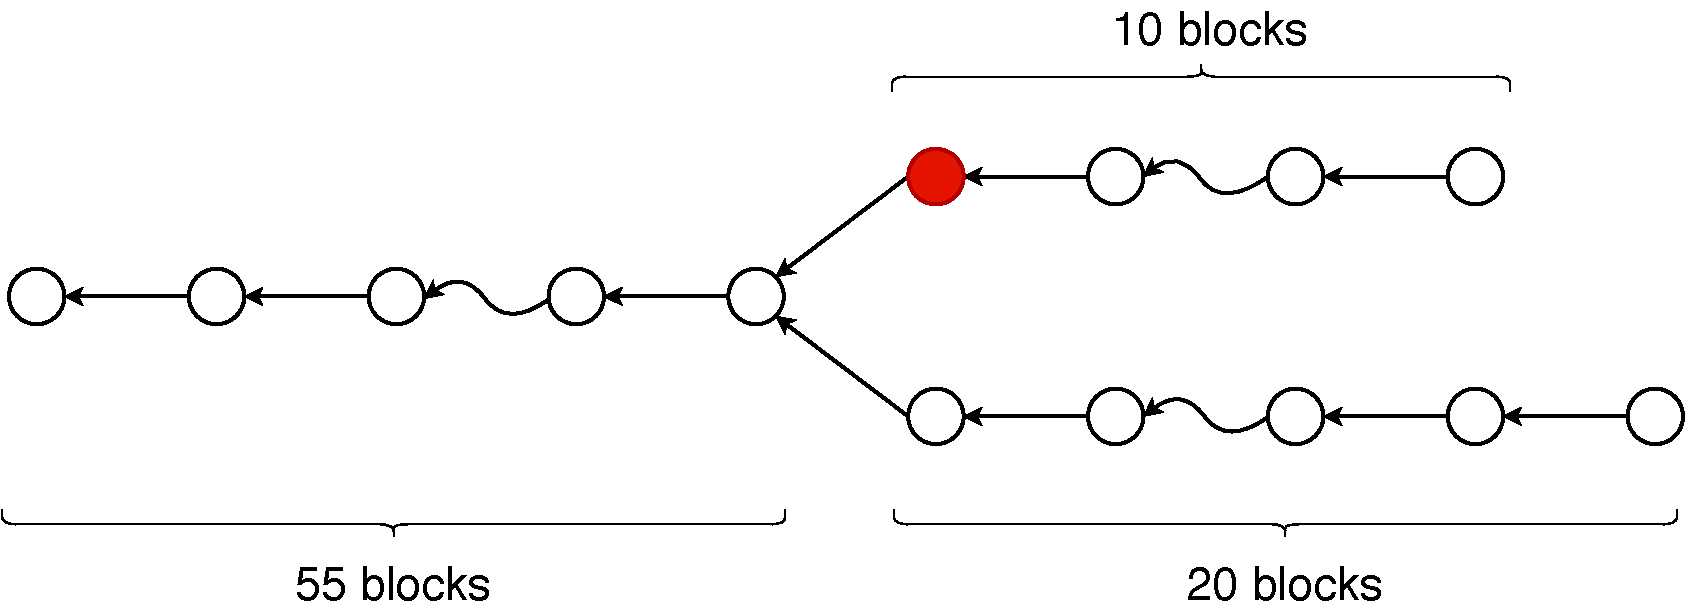
\includegraphics[width=10cm]{./images/proofs_65-10+20.pdf}
    \caption{The red block indicates the block of interest. Curved connections
        imply intermediate blocks. The adversary creates a proof for an event
        that does not exist in the honest chain}
    \label{figure:proofs_65-10+20}
\end{figure}

\begin{table}[H]
    \centering
    \begin{tabular}{@{}lccll@{}}
        \toprule
        \multicolumn{1}{c}{\textbf{Submit function}} & \textbf{gas usage}    \\ \midrule
        validate Interlink  & \multicolumn{1}{r}{   465,604} \\
        \\
        \\
        store proof         & \multicolumn{1}{r}{ 1,044,705} \\
        store DAG           & \multicolumn{1}{r}{ 3,168,612} \\
        store ancestors     & \multicolumn{1}{r}{ 4,995,289} \\
        evaluate predicate  & \multicolumn{1}{r}{   306,433} \\
        delete ancestors    & \multicolumn{1}{r}{    45,137} \\
        \midrule
        Sum                 & \multicolumn{1}{r}{10,025,780} \\
        \bottomrule
    \end{tabular}
    \quad
    \begin{tabular}{@{}lccll@{}}
        \toprule
        \multicolumn{1}{c}{\textbf{Contest function}} & \textbf{gas usage} \\ \midrule
        validate Interlink  & \multicolumn{1}{r}{   485,751} \\
        find LCA            & \multicolumn{1}{r}{ 1,255,523} \\
        compare proofs      & \multicolumn{1}{r}{   447,130} \\
        store proof         & \multicolumn{1}{r}{   304,845} \\
        update DAG          & \multicolumn{1}{r}{ 1,836,578} \\
        store ancestors     & \multicolumn{1}{r}{ 5,584,173} \\
        evaluate predicate  & \multicolumn{1}{r}{   390,307} \\
        delete ancestors    & \multicolumn{1}{r}{    57,023} \\
        \midrule
        Sum                 & \multicolumn{1}{r}{10,361,330} \\
        \bottomrule
    \end{tabular}
    \caption{Execution for proof of 75 blocks}
    \label{table:old_gas_usage}
\end{table}


In this scenario, the original proof is created by an adversary for an event
that does not exist in the honest chain. The proof is contested by an honest
party. We selected this configuration because it includes both phases
(submit and contest) and provides full code coverage of each phase since all
underlying operations are executed and no early returns occur.

For a chain of 75 blocks, each phase of the contract needed more than 10
million gas units. Although the size of this test chain is only a very small
faction of the size of a realistic chain, the gas usage already exceeds the
limit of Ethereum blockchain, which is slightly below 10 million. In
particular, the submit of a 500,0000-blocks chain demands 47,280,453 gas. In
Figure \ref{figure:old_gas_per_chain_proof}, we show gas consumption for submit
phase for different chain sizes and their corresponding proofs sizes. We
demonstrate results for chains sizes from 100 blocks (corresponding proof size
25) to 500,000 blocks (corresponding to proof size 250).

The linear relation displayed in Figure \ref{figure:old_gas_per_proof} implies
that the gas consumption of the verifier is determined by the size of the
proofs. As shown in Figure \ref{figure:size_of_nipopows} \todo{insert figure
for proof size with relation to the chain in Background}, the size of the
proofs grows logarithmically to the size of the chain, and this is also
reflected to the gas consumption curve.

\begin{figure}[ht]
\centering
\begin{subfigure}[b]{.49\textwidth}
\begin{tikzpicture}
    \begin{axis}[
        scaled y ticks = true,
        scaled x ticks = false,
        grid=major,
        width=\textwidth,
        xlabel={Chain size},
        ylabel={Gas consumption}
        ]
    \addplot table [col sep=comma] {data/old_gas_per_chain.csv};
\end{axis}
\end{tikzpicture}
\centering
\caption{Gas consumption per chain size}
\label{figure:old_gas_per_chain}
\end{subfigure}
\begin{subfigure}[b]{.49\textwidth}
\begin{tikzpicture}
    \begin{axis}[
        scaled y ticks = true,
        scaled x ticks = false,
        grid=major,
        width=\textwidth,
        xlabel={Proof size},
        ylabel={Gas consumption}
        ]
    \addplot table [col sep=comma] {data/old_gas_per_proof.csv};
\end{axis}
\end{tikzpicture}
\centering
\caption{Gas consumption per proof size}
\label{figure:old_gas_per_proof}
\end{subfigure}
\caption{Gas consumption with respect to chain and corresponding proof size}
\label{figure:old_gas_per_chain_proof}
\end{figure}



\begin{wraptable}{h}{6.0cm}
    \centering
    \begin{tabular}{@{}lccll@{}}
        \toprule
        \multicolumn{1}{c}{\textbf{Chain size}} & \textbf{Toll}  \\ \midrule
        \multicolumn{1}{r}{    100} & \multicolumn{1}{r}{ 12.43 \euro{} } \\
        \multicolumn{1}{r}{    500} & \multicolumn{1}{r}{ 16.14 \euro{} } \\
        \multicolumn{1}{r}{  1,000} & \multicolumn{1}{r}{ 23.79 \euro{} } \\
        \multicolumn{1}{r}{ 10,000} & \multicolumn{1}{r}{ 33.47 \euro{} } \\
        \multicolumn{1}{r}{ 50,000} & \multicolumn{1}{r}{ 44.03 \euro{} } \\
        \multicolumn{1}{r}{100,000} & \multicolumn{1}{r}{ 45.65 \euro{} } \\
        \multicolumn{1}{r}{500,000} & \multicolumn{1}{r}{ 49.88 \euro{} } \\
        \bottomrule
    \end{tabular}
    \caption{Tolls for different chain sizes. Gas price is Gwei}
    \label{table:old_cost_in_fiat}
\end{wraptable}


\paragraph{Pricing}

So far, we have shown that the verifier is not applicable to the real
blockchain due to extensive gas usage, exceeding the build-in limitation the
Ethereum blockchain by far. While Ethereum adapts to community demands and
build-in parameters can change, it seem improbable to ever incorporate such a
high block gas limit. However, even in this extreme case, the verifier would
still be impractical due to the high cost of the operations in fiat. We call
this amount \emph{toll}, because it is the cost of using the "bridge" between
two blockchains. We list these tolls in Table \ref{table:old_cost_in_fiat}. For
this price, we used gas price equal to 5 Gwei, which is considered an average
amount to complete transactions. With this gas price, the probability
approximately that the transaction will be included in one of the next 200
blocks is 33\%. Note that average gas price will not be sufficient for
contesting phase, and it has to be performed with higher gas price because of
the limited contesting period. We will later analyze thoroughly the entire
spectrum of gas prices and tolls for realistic usage of both submit and contest
phases.

\subsection{Security Analysis}

\subsubsection{Pre-mining} We observed that the verifier is vulnerable to
pre-mining(ref). By definition, a NIPoPoW is structurally correct if two
properties are satisfied:

\begin{enumerate}[(a)]

\item The interlink structure of all blocks is correct. This is to prevent
    adversaries from injecting blocks that do not exist in the original
    blockchain.

\item The first block of proof is $genesis$. This is to prevent adversaries
    from create coins before blockchain are advertised at the public network.

\end{enumerate}

The second property is not verified in the previous work, exposing the verifier
to pre-mining attacks. We can easily mitigate this vulnerability by
initializing the smart contract with the $genesis$ block of the blockchain we
will use and add an assertion in submit and contest phase that proofs need to
satisfy property (b). The needed changes are shown in
Algorithms~\ref{algo:avoid_premining_ctor}
and~\ref{algo:avoid_premining_submit}.

\begin{algorithm}[H]

    \caption{\label{alg:avoid-premining}The \textsf{NIPoPoW} client mitigation
    to premining attack}
    \begin{algorithmic}[1]

    \Contract{crosschain}
    \State $\textsf{events} \gets \bot$; $\genesis \gets \bot$
    \State $\textsf{DAG} \gets \bot$; $\textsf{ancestors} \gets \bot$
    \Function{\sf initialize}{$\genesis_{remote}$}
        \State $\genesis$ $\gets \genesis_{remote}$
        \Comment{initialize with the genesis of the underlying chain}
    \EndFunction
    \Function{\sf submit}{$\pis$, $e$}
        \State \textsf{require}($\pis$[0] = $\genesis$)
        \Comment{assert correct genesis}
        \State \textsf{require}($\textsf{events$[e]$} = \bot$)
        \State \textsf{require}($\textsf{valid-interlinks}(\pi)$)
        \State \textsf{events$[e].\pi$} $\gets$ $\pis$
        \State \textsf{DAG} $\gets$ \textsf{DAG} $\cup$ $\pi$
        \State \textsf{ancestors} $\gets$ \textsf{find-ancestors(DAG, $\pi$[-1])}
        \State \textsf{require}(\textsf{evaluate-predicate}(\textsf{ancestors}, e))
        \State \textsf{ancestors} $=$ $\bot$
        \EndFunction
    \Function{\sf contest}{$\pic$, $e$}
        \State \textsf{require}($\pic$[0] = $\genesis$)
        \Comment{assert correct genesis}
        \State \textsf{require}(\textsf{events}$[e]$ $\ne$ $\bot$)
        \State \textsf{require}(\textsf{valid-interlinks}($\pic$))
        \State $lca$ = \textsf{find-lca}($\textsf{events}[e].\pi$, $\pic$)
        \State \textsf{require}($\pic$ $\geq_m$ $\textsf{events}[e].\pi$)
        \State \textsf{DAG} $\gets$ \textsf{DAG} $\cup$ $\pic$
        \State \textsf{ancestors} $\gets$
        \textsf{find-ancestors}($\textsf{DAG}$, $\textsf{events}[e].\pi$[-1])
        \State \textsf{require}($\neg$\textsf{evaluate-predicate}(\textsf{ancestors}, $e$))
        \State \textsf{ancestors} $=$ $\bot$
        \State \textsf{events$[e]$} $\gets$ $\bot$
    \EndFunction
    \EndContract
    \vskip8pt
    \end{algorithmic}
\end{algorithm}



\subsubsection{Score Calculation}

During our tests, we observed that the calculation of proofs score was
incorrect. The score of each level is needed to determine which proof
represents the chain with the most Proof of Work. Between two proofs, we only
need to calculate the score starting from their $lca$ until the tip of each
proof. Different levels are needed because the $lca$ between two proofs is only
known when the contesting proof is submitted. The security parameter $m$ needs
to be satisfied for every sub-proof $\pi[:lca]$. We ensure that this is $true$
by creating proofs of multiple levels, so that security parameter $m$ applies,
disregarding $lca$'s position.

\todo{Figure for the need of multiple levels}

Each block has a level, calculated as describe in Section(ref)
\[ level = getLevel(block) \]
Consequently, each level of the proof consists of a number of blocks
$n_{level}$. This number is the sum of blocks of level $\geq$ $level$, i.e.\
block of level $l$ are also blocks of levels $l-1$, $l-2$, etc. The
score of each level is computed as:

\[score_{level} = 2^{level} \times n_{level}\]

After running out tests for the previous implementation, we observed that
function $getLevel(block)$ of the contract was returning $block.level-1$
instead of $block.level$ resulting to incorrect score computation. This can
prevent an honest party from successfully contesting an adversarial proof,
making the contract insecure. The function was refined to return the correct
value.

\section{Storage Elimination}
\todo{Should this be a new section?}

As mentioned above, the bottleneck we had to eliminate was the extensive usage
of storage. We created a new architecture that allow us to discard all
expensive store operations and utilize memory instead. This led to massive
decrease of gas consumption. In this section, we present the difference in gas
usage between storage and memory utilization, and how a NIPoPoW verifier can be
implemented in Solidity without persisting proofs.

\subsection{Storage vs Memory}

We will first demonstrate the difference in gas usage between storage and
memory for a smart contract in Solidity. Suppose we have the following simple
contract:

\lstinputlisting[style=customc, captionpos=b, label={listing:storage_memory},
caption={Solidity test for storage and memory}]{code/StorageVsMemory.sol}
\todo{Highlight code}

Function \texttt{withStorage()} populates an array saved in storage and
function \texttt{withMemory()} populates an array saved in memory. We
initialize the sizes of the arrays by passing the variable \texttt{size} to the
contract constructor. We run this piece of code for \texttt{size} from 1 to
100. The results are displayed at Figure~\ref{figure:memory_vs_storage}. For
\texttt{size} = 100, the gas expended is 53,574 gas units using memory and
2,569,848 using storage which is almost 50 times more expensive. This code was
compiled with Solidity version 0.6.6 with optimizations enabled\footnote{This
version of Solidity compiler, which was the latest at the time this paper was
published, did not optimize-out any of the variables.}. The EVM we used  was
Ganache at the latest Constantinople(ref) fork. It is obvious that if there is
the option to use memory instead of storage in the design of smart contracts,
the choice of memory greatly benefits the users.

\begin{figure}
\centering
\begin{tikzpicture}
    \begin{axis}[
        y tick label style={/pgf/number format/.cd,%
          set thousands separator={,},
          fixed},
        legend pos=north west,
        scaled y ticks = false,
        grid=major,
        xlabel={Array size},
        ylabel={Gas consumption}]
    \addplot table [mark=none, col sep=comma] {data/storage.csv};
    \addplot table [mark=none, col sep=comma] {data/memory.csv};
    \legend{$storage$,$memory$};
\end{axis}
\end{tikzpicture}
\caption{Gas consumption for memory and storage}
\label{figure:memory_vs_storage}
\end{figure}


\subsection{Making use of calldata}

In previous work we needed to store submitted proofs in order to proceed to
contest. In this subsection we show an approach to securely verify proofs
without utilizing the persistent storage of the smart contract.

The rationale is to demand from the caller to provide two proofs to the
contract during contest phase: (a) $\pi_{exist}$, which is a copy of the
originally submitted proof $\pi_{orig}$, and (b) $\pi_{cont}$, which is the
contesting proof. Proof $\pi_{orig}$ can be retrieved by observing contract's
\textit{calldata}. We prevent an adversary from malforming $\pi_{exist}$ by
storing the hash of $\pi_{orig}$ to contract's state during submit phase and
then verifying that $\pi_{exist}$ has the same hash. The operation of hashing
the proof and storing the digest is cheap\footnote{By setting $k=6$, $m$ = 13,
a proof for the entire Bitcoin blockchain consists of less than 300
superblocks. The hashing of such a proof costs approximately 300,000 gas
units.} as shown in figure~\ref{figure:hash_proof_gas}. We calculate the digest
of the proof by:

\[\texttt{digest = sha256(abi.encodePacked(proof))}\] The size of the digest of
a hash is 32 bytes. To persist such a small value in contract's memory only
adds a constant, negligible cost overhead to our implementation.

\begin{figure}
\centering
\begin{tikzpicture}
    \begin{axis}[
        y tick label style={/pgf/number format/.cd,%
          set thousands separator={,},
          fixed},
        legend pos=north west,
        scaled y ticks = false,
        grid=major,
        xlabel={Proof size},
        ylabel={Gas consumption}]
    \addplot table [col sep=comma] {data/hash_proof_gas.csv};
    \legend{sha256 gas cost};
\end{axis}
\end{tikzpicture}
\caption{Gas consumption for hashing proofs and storing digest}
\label{figure:hash_proof_gas}
\end{figure}



\subsection{Removing DAG and ancestors}

As shown in table~\ref{table:old_gas_usage}, the most demanding operation is
the creation and population of DAG and ancestors. In this subsection we show
how these two structures can be discarded from the verifier.

\subsubsection{Using subset} Our first realization was that instead of storing the
DAG of $\pi_{exist}$, $\pi_{cont}$, we can require

\[ \pi_{exist}\{:lca_{e}\} \subseteq \pi_{cont}\{:lca_{c}\} \]
where $lca_{e}$ and $lca_{c}$ are the indices of the $lca$ block in
$\pi_{exist}$, and $\pi_{cont}$, respectively. This way we avoid
the demanding need of composing auxiliary structures DAG and ancestors
on-chain. The implementation of \texttt{subset} is displayed in
listing~\ref{listing:subset}. The complexity of the function is
\[ \mathcal{O}(\mid\pi_{exist}[:lca_{e}]\mid + \mid\pi_{cont}[:lca_{c}]\mid) \]

\lstinputlisting[style=customc, captionpos=b, label={listing:subset},
caption={Implementation of subset}]{code/Subset.sol}

\begin{figure}[ht]
\begin{subfigure}{.5\textwidth}
  \centering
  % include first image
  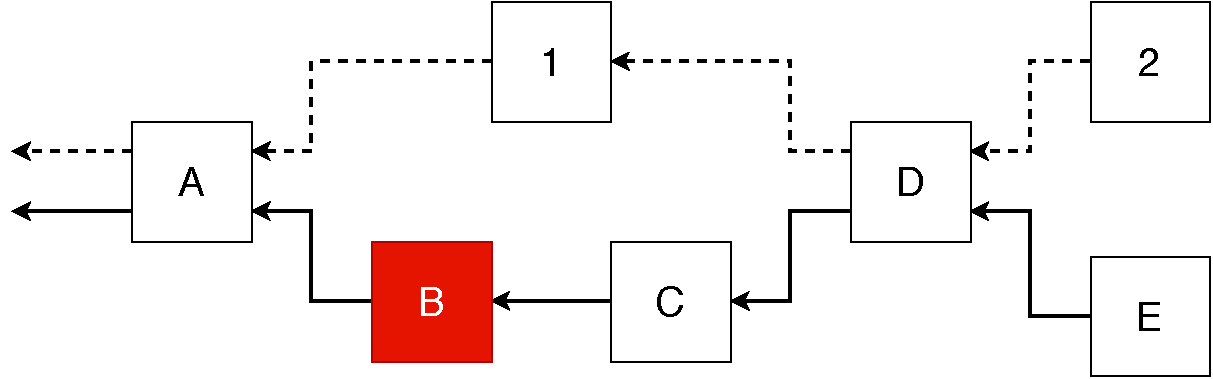
\includegraphics[width=6cm]{../images/Subset_1.pdf}
  \caption{Valid $\pi_{cont}$ before using subset}
  \label{figure:DAG_usage}
\end{subfigure}
\begin{subfigure}{.5\textwidth}
  \centering
  % include second image
  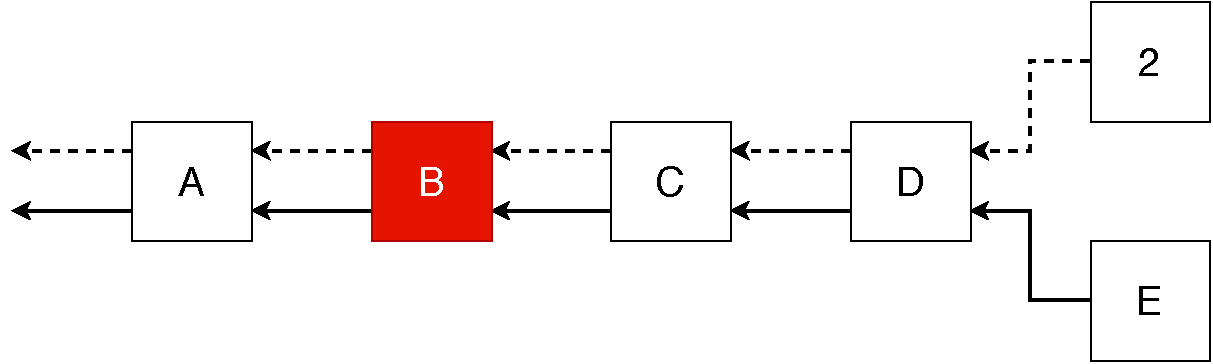
\includegraphics[width=6cm]{../images/Subset_2.pdf}
  \caption{Valid $\pi_{cont}$ after using subset}
  \label{figure:DAG_usage}
\end{subfigure}
\caption{Blocks connected with solid lines indicate $\pi_{exist}$ and blocks
connected with dashed lines indicate $\pi_{cont}$}
\label{fig:fig}
\end{figure}


The gas consumption difference between $subset$ and $DAG + ancestors$ is
displayed at figure~\ref{figure:DAG_vs_subset}. $Subset$ solution is
approximately 2.7 times more efficient.

\begin{figure}
\centering
\begin{tikzpicture}
    \begin{axis}[
        y tick label style={/pgf/number format/.cd,%
          set thousands separator={,},
          fixed},
        legend pos=north west,
        scaled y ticks = false,
        grid=major,
        xlabel={Proof size},
        ylabel={Gas consumption x 1.000}]
    \addplot table [col sep=comma] {data/DAG_ancestors.csv};
    \addplot table [col sep=comma] {data/subset.csv};
    \legend{$DAG+ancestors$,$Subset$};
\end{axis}
\end{tikzpicture}
\caption{Gas consumption for DAG+ancestors and subset}
\label{figure:DAG_vs_subset}
\end{figure}


\subsubsection{Subset complexity and limitations} Requiring $\pi_{exist}$ to be a subset of
$\pi_{cont}$ greatly reduces gas, but the complexity of the $subset$ algorithm
is high since both proofs have to be iterated from genesis to their respective
$lca$ index. Generally, we expect for an adversary to provide a proof of a
chain that is a fork of the honest chain at some point relatively close to the
tip. This is due to the fact that the ability of an adversary to sustain a fork
chain is exponentially weakened as the honest chain progresses.  This means
that the length of $\pi$, $\mid\pi\mid$ is be considerably close to
$\mid\pi[:lca]\mid$, and the complexity of \texttt{subset()} is effectively
$\mathcal{O}(2\mid\pi\mid)$.

In realistic cases, where the $lca$ lies around index 250 of the proof, the gas
cost of \texttt{subset()} is approximately 20,000,000 gas units, which makes it
inapplicable for real blockchains since it exceeds the block gas limit of
the Ethereum blockchain by far.

\subsubsection{Position of block of interest}

By analyzing the benefits and trade-offs of $subset$, we concluded that there
is a more efficient way to treat storage elimination. In general, the concept
of $subset$ facilitated the case in which the block of interest belongs in the
sub-proof $\pi_{exist}[:lca_{e}]$. But in this case, both $\pi_{exist}$ and
$\pi_{cont}$ contain the block of interest at some index, as can be seen in
figure~\ref{figure:after_subset}. Consequently, $\pi_{cont}$ cannot contradict
the existence of the block of interest and the predicate is evaluated $true$
for both proofs. This means that if (a) $\pi_{exist}$ is structurally correct
and (b) the block of interest is in $\pi_{exist}[:lca_{e}]$, then we can safely
conclude that contesting with $\pi_{cont}$ is redundant. Therefore,
$E_{contest}$ can simply send $\pi_{cont}$[lca:] to the verifier. The
truncation of $\pi_{cont}$ to $\pi_{cont}[lca_{c}:]$ can be easily addressed
from $E_{cont}$, since $\pi_{exist}$ is accessible from the contract's
calldata and both proofs can be iterated off-chain.

\newcommand*{\exist}{$\pi_{exist}$}
\newcommand*{\cont}{$\pi_{cont}^{tr}$}

\subsubsection{Disjoint proofs}

We will refer to the truncated contesting proof as $\pi_{cont}^{tr}$ and to
$lca_{e}$ simply as $lca$. For the aforementioned, the following statements are
true:

\begin{enumerate}[(a)]
    \item  $\pi_{exist}[0]$ = $genesis$
    \item  $\pi_{exist}[lca]$ = $\pi_{cont}^{tr}[0]$
\end{enumerate}

The requirement that needs to be satisfied is
\[\pi_{exist}\{lca+1:\} \cap \pi_{cont}^{tr}\{1:\} = \emptyset \]

The implementation of this operation is shown in
listing~\ref{listing:disjoint}.

\lstinputlisting[style=customc, captionpos=b, label={listing:disjoint},
caption={Implementation for disjoint proofs}]{code/Disjoint.sol}

The complexity of \texttt{disjoint()} is
\[ \mathcal{O}(\mid\pi_{exist}[lca_{e}:]\mid \times
\mid\pi_{cont}^{tr}\mid) \]

\section{Fixing vulnerabilities and restricting gas usage}

% \begin{itemize}
%
%     \item
%         This is not vulnerable to DOS attacks
%
% \end{itemize}
